\documentclass[a0,landscape]{a0poster}
%%%Load packages
\usepackage{symbols}
\usepackage{amssymb,amsmath,amsthm,amsfonts}
\usepackage{mathrsfs}
\usepackage{multicol} 			%3-column layout
\usepackage[absolute]{textpos}
\usepackage{caption, subcaption}
\usepackage{float}
%\usepackage{pstcol}
\usepackage{boxedminipage}
\usepackage{hyperref}
\usepackage[absolute]{textpos}
\usepackage{xcolor,tabularx}
\usepackage{algorithm, algorithmicx, algpseudocode}
\usepackage{xcolor}
\usepackage{array}
\usepackage{booktabs}
\definecolor{ForestGreen}{RGB}{34,139,34}
\usepackage{tcolorbox}
\usepackage{tikz}
\usetikzlibrary{calc,positioning}
\newtheorem*{theorem}{Theorem}
\usepackage{etoolbox}
\patchcmd{\thebibliography}{\section*{\refname}}{}{}{}

\usepackage[left=0cm,right=0cm,bottom=0cm,top=0cm]{geometry}

\definecolor{JHUblue}{RGB}{80,0,0}
\definecolor{JHUGray}{RGB}{255,255,255}
\definecolor{headingcol}{rgb}{1,1,1}			%Colour of main title
\definecolor{boxcol}{rgb}{0.05,0.2,0.33}		%Edge-colour of box and top banner
\definecolor{boxcol2}{rgb}{0.2,0.32,0.44}		%Edge-colour of box and top banner
\fboxsep=1.1cm							%Padding between box and text
\setlength{\columnsep}{2cm}				%Set spacing between columns

\let\Textsize\large

\def\heading#1{\sffamily\begin{flushleft} \LARGE\sffamily{\color{DarkBlue} #1}
		\vspace{4mm}
\end{flushleft}\large } %
%%%Format title
\makeatletter							%Needed to include code in main file

\renewcommand\@maketitle{%
\null									%Sets position marker
{
\color{headingcol}\sffamily\VeryHuge		%Set title font and colour
\@title \par
}
\par 
}
\makeatother

\title{Learning Joint and Individual Structure \\in Network Data with Covariates
	
}
\TPGrid[50mm,50mm]{23}{12}

\usepackage{exscale}

%%%Define "Section" environment for framed boxes
%%%Usage: \begin{Section}{Name} blah blah blah \end{Section}
\newenvironment{Section}[2]				%Environment takes one argument
%%%Opening
{
	\par
	\vspace{1cm}
	\fcolorbox{JHUblue}{JHUblue}{\begin{minipage}{\columnwidth}{\sffamily\LARGE\color{white}#1 }\end{minipage}}	%Draws solid colour box around title
	%Typesets section name
	\par\nobreak 
	
	\fcolorbox{JHUblue}{white}{\parbox{ \columnwidth\fboxsep\fboxrule\sffamily\large}{%
			%%%Closing 
			#2}}
	\vspace{0.5cm}						%Add spacing below box
} 


\begin{document}
		
\hspace{-1cm}								%Align with edge of page, not margin
\colorbox{JHUblue}{

	\hspace{1cm}
	\begin{minipage}[c]{0.75\linewidth}
	\vspace{-2cm}
	\maketitle
	\vspace{-2cm}
	\end{minipage}
	\begin{minipage}[c]{0.3\linewidth}
		\vspace{-1cm}
		\scalebox{1.2}{
\includegraphics {Images/TAM-LogoBox}} 
		\vspace{-1cm}
	\end{minipage}
}
\\%[-2pt]

\vspace{-0.1cm}

\hspace{-1cm}\colorbox{JHUGray}{\hspace{1cm}\begin{minipage}{1189mm}					%Minipage for title contents
{\vspace{0cm}
\color{white}\sffamily\huge		%Set title font and colour
Carson James$^{1}$, Dongbang Yuan$^{1}$, Jes\'us Arroyo$^{1}$, Irina Gaynanova$^{1}$\\
\textit{$^{1}$Texas A\&M University}}
\end{minipage}}




\hspace{0.2cm}\begin{minipage}{0.97\textwidth}
	\centering
	%%%%%%%%%%%%%%%%% FIRST COLUMN %%%%%%%%%%%%%%%%%%%%%%%%%%%%%%%%%%%%%%%%%%%%%%
	\begin{minipage}[t]{0.3\textwidth}
		\begin{Section}{Modeling multiple heterogeneous networks}{
				\fcolorbox{white}{white}{\parbox{\textwidth}{\vspace{1cm}\centering\parbox{0.9\textwidth}
						{\textbf{Motivation:} 
							\begin{itemize}
								\item We present the \emph{common subspace independent-edge} (COSIE) model which describes a 
								collection of networks with a shared latent structure on the vertices but potentially different connectivity
								patterns for each graph \cite{arroyo2019inference}.
								\item COSIE encompasses many other popular network representations, including the stochastic blockmodel
								\item A joint spectral embedding - the \emph{multiple adjacency spectral embedding}- leads to consistent estimation that is computationally efficient
								\item MASE estimates yield state-of-the-art performance on subsequent inference tasks, including dimensionality reduction, hypothesis testing and community detection
							\end{itemize}
				}}}
			\vspace{1cm}\\
				\begin{minipage}{0.58\textwidth}
					%\textbf{Motivation}
					\begin{itemize}
						\item Models for multiple network data are critical in
						statistical network theory and across multiple domains, including neuroscience, biology and the social sciences.
						\item  Challenges in modeling graph differences while retaining sufficient model simplicity to render
						estimation feasible.
						\item Existing models require strong assumptions that limit their flexibility or scalability
					\end{itemize}
				\end{minipage}
				\begin{minipage}{0.38\textwidth}
					\centering
					{\small Difussion MRI brain connectomes from the HNU1 data\par}
					%\includegraphics[width=0.8\textwidth]{../Presentation/Images/HNU1-graphs-square}
				\end{minipage}
				
				\definecolor{verylightgray}{RGB}{211,211,211}
				
			}
		\end{Section}
	
	\begin{Section}{Common subspace independent edge (COSIE) model}{
			%\textbf{Setting:}
			\begin{itemize}
				\item Consider a sample of $m$ graphs with $n$ labeled nodes.
				\item Denote the graphs by their adjacency matrices $\bA^{(1)}, \ldots, \bA^{(m)}\in\{0,1\}^{n \times n}$
				\item Each graph $\bA^{(i)}$ is modeled as independent-edge  with parameter $\bP^{(i)}\in\real^{n\times n}$
				\[\bA^{(i)}_{uv} \sim \operatorname{Ber}(P_{uv}^{(i))}). \]
			\end{itemize}
			\textbf{COSIE model}
			\begin{itemize}
				\item The sample of graphs is jointly distributed according to the COSIE model if
				\begin{equation*}
					\bP^{(i)} : = \bV\bR^{(i)}\bV^T.
				\end{equation*}
				\item $\bV\in\real^{n\times d}$ is a matrix with orthogonal columns, with its rows representing vertex latent positions
				\item $\bR^{(i)}\in\real^{d\times d}$ is a score matrix, potentially different for each graph
				\item The parameter $d$ controls the complexity of the model
			\end{itemize}
			
		}
		\end{Section}
	\end{minipage}
	\hfill
	%%%%%%%%%%%%%%%%% Second COLUMN %%%%%%%%%%%%%%%%%%%%%%%%%%%%%%%%%%%%%%%%%%%%%%
	\begin{minipage}[t]{0.32\textwidth}
		\begin{Section}{Multiple adjacency spectral embedding (MASE)}{
			
			\begin{enumerate}
				\item For each $i\in[m]$, obtain the $d$-dimensional unscaled \emph{adjacency spectral embedding} of $\bA^{(i)}$, denoted by $\hat{\bV}\in\real^{n\times d}$ and corresponding to the $d$ leading eigenvectors
				\item Let $\hat{\bU} = \left( \hat{\bV}^{(1)} \ \cdots \ \hat{\bV}^{(m)}\right)$ be the $n\times (md)$ matrix of concatenated ASEs.
				\item Let $\hat{\bV}\in\real^{n\times d}$ be the matrix containing the $d$ leading left singular values of $\hat{\bU}$.
				\item For each $i\in[m]$, set $\hat{\bR}^{(i)} = \hat{\bV}^T\bA^{(i)}\hat{\bV}$.
			\end{enumerate}		
			{\centering
				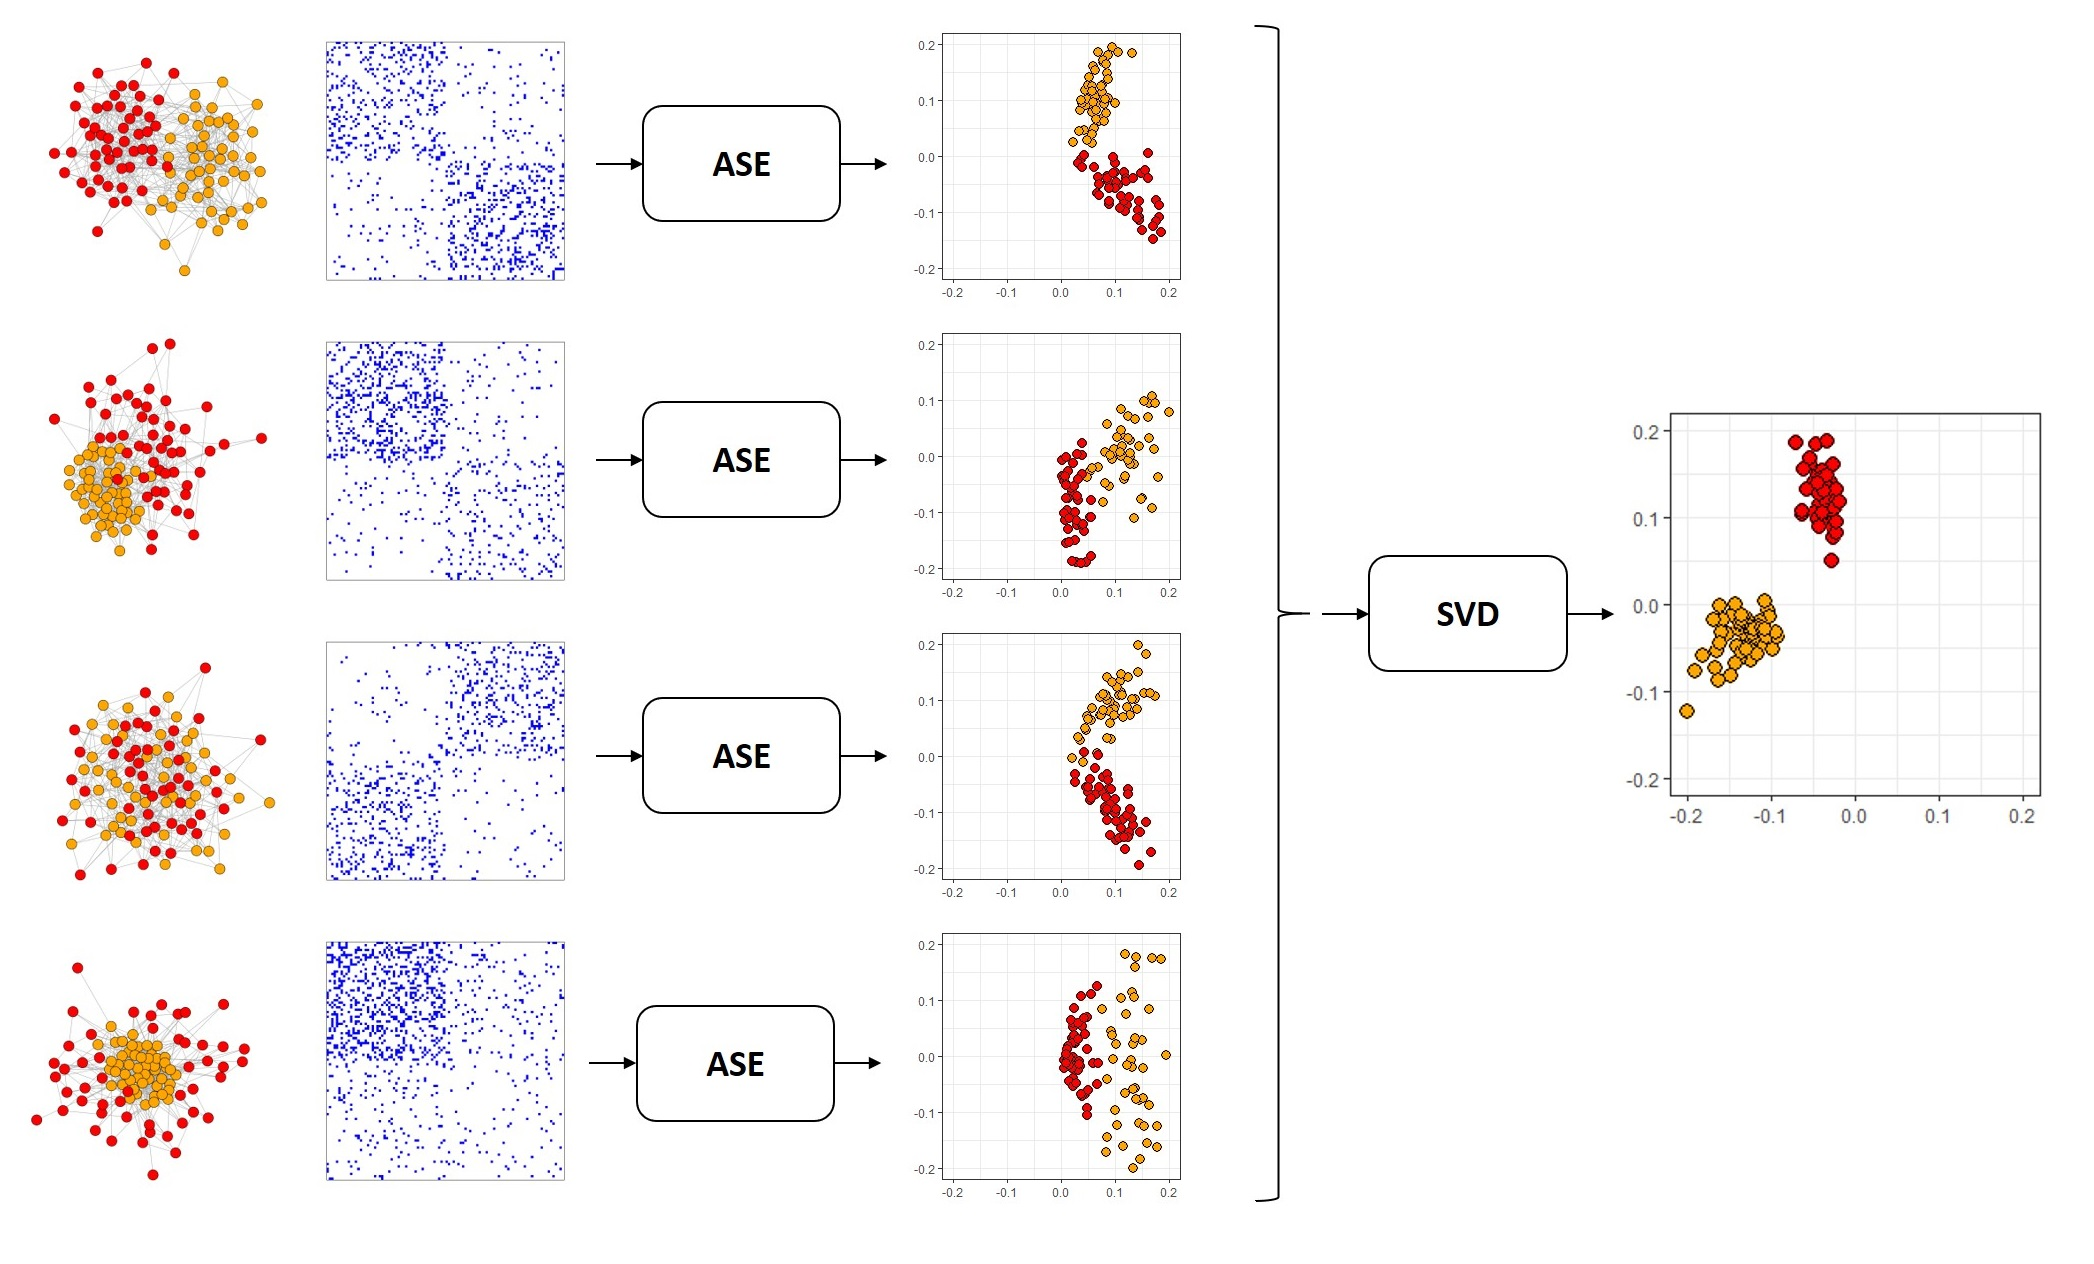
\includegraphics[width=0.99\textwidth]{Images/mase1}
			}
			
		}
		\end{Section}
		\begin{Section}{Theoretical properties}{
				\textbf{Consistency of common invariant subspace estimator}
				\begin{itemize}
					\item Under some assumptions on the smallest eigenvalue of the score matrices and on the sparsity of the graphs, the estimate of $\bV$ obtained by MASE satisfies
					\begin{equation*}
					\e\left[\min_{\bW \in\mathcal{O}_d} \left\| \hat{\bV} - \bV\bW \right\|\right] \lesssim \sqrt{\frac{d}{mn}} + \frac{\sqrt{d}}{n}.
					\end{equation*}
					\item When $\bV$ has only $d$ different rows, COSIE is equivalent to the stochastic blockmodel, and $k$-means clustering expected error in community detection is $O\left(\sqrt{\frac{d}{m}} + \frac{1}{\sqrt{n}}\right)$.
				\end{itemize}
				\textbf{Asymptotic normality of the score matrices}
				\begin{itemize} 					
				\item The entries of the estimated score matrices $\hat{\bR}^{(i)}$ are asymptotically normally distributed, in particular, as the size of the graphs $n$ increases
				\begin{equation*}
					\frac{1}{\sigma_{ijk}}\left( \hat{\bR}^{(i)}  - \bW\bR^{(i)}\bW^T + 	\bH\right)_{jk} \overset{d}{\rightarrow} \mathcal{N}(0,1)
				\end{equation*}
				where $\sigma_{ijk}=O(1)$,  $\e[\|\bH\|_F] = O(d/\sqrt{m})$ and $\|\bR^{(i)}\|_F\rightarrow\infty$.
				\end{itemize}
			}
		\end{Section}
	\end{minipage}
	\hfill
	%%%%%%%%%%%%%%%%% THIRD COLUMN %%%%%%%%%%%%%%%%%%%%%%%%%%%%%%%%%%%%%%%%%%%%%%
	\begin{minipage}[t]{0.3\textwidth}
		\begin{Section}{Brain network analysis}{
				\begin{minipage}{0.39\textwidth}
					\textbf{HNU1 data}
					\begin{itemize}
						\item 300 graphs constructed from diffusion magnetic resonance imaging (dMRI), with $n=200$ nodes
						\item 30 different healthy subjects, and 10 graphs per subject
						\item \textbf{Goal:} identify differences and similarities between graphs
					\end{itemize}
				    \textbf{Dimensionality reduction}
				    \begin{itemize}
						\item The vertex embedding $\hat{\bV}$ obtained by MASE (top figure) reflects the anatomical location of the vertices in the brain.
						\item A multidimensional scaling of the distance between the score matrices $\{\bR^{(i)}\}_{i=1}^{300}$ (bottom figure) puts graphs from the same subject closer to each other
					\end{itemize}
				\end{minipage}\hfill
				\begin{minipage}{0.59\textwidth}
					{\centering
						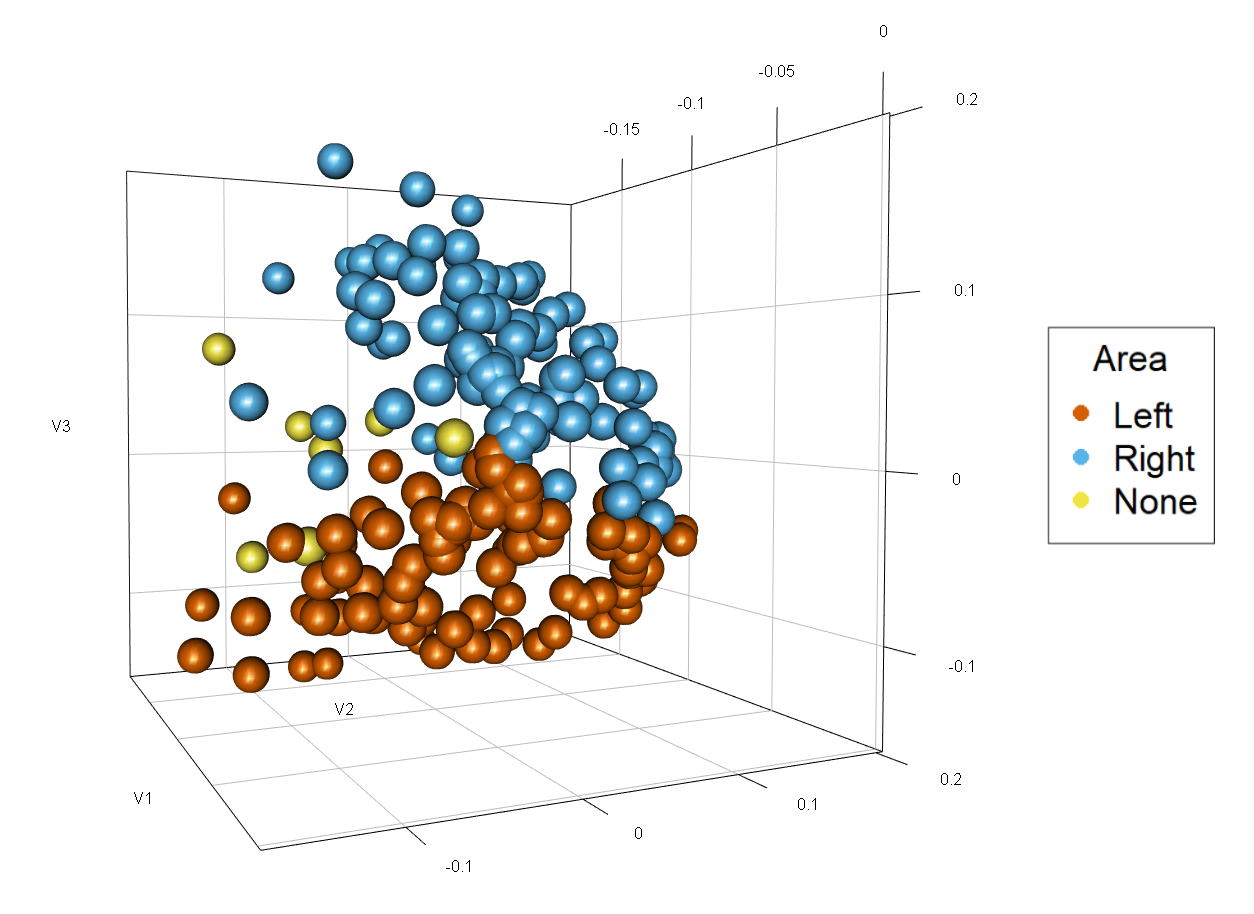
\includegraphics[width=\textwidth]{Images/HNU1-latentpositions-plot}
					}
					{\centering
						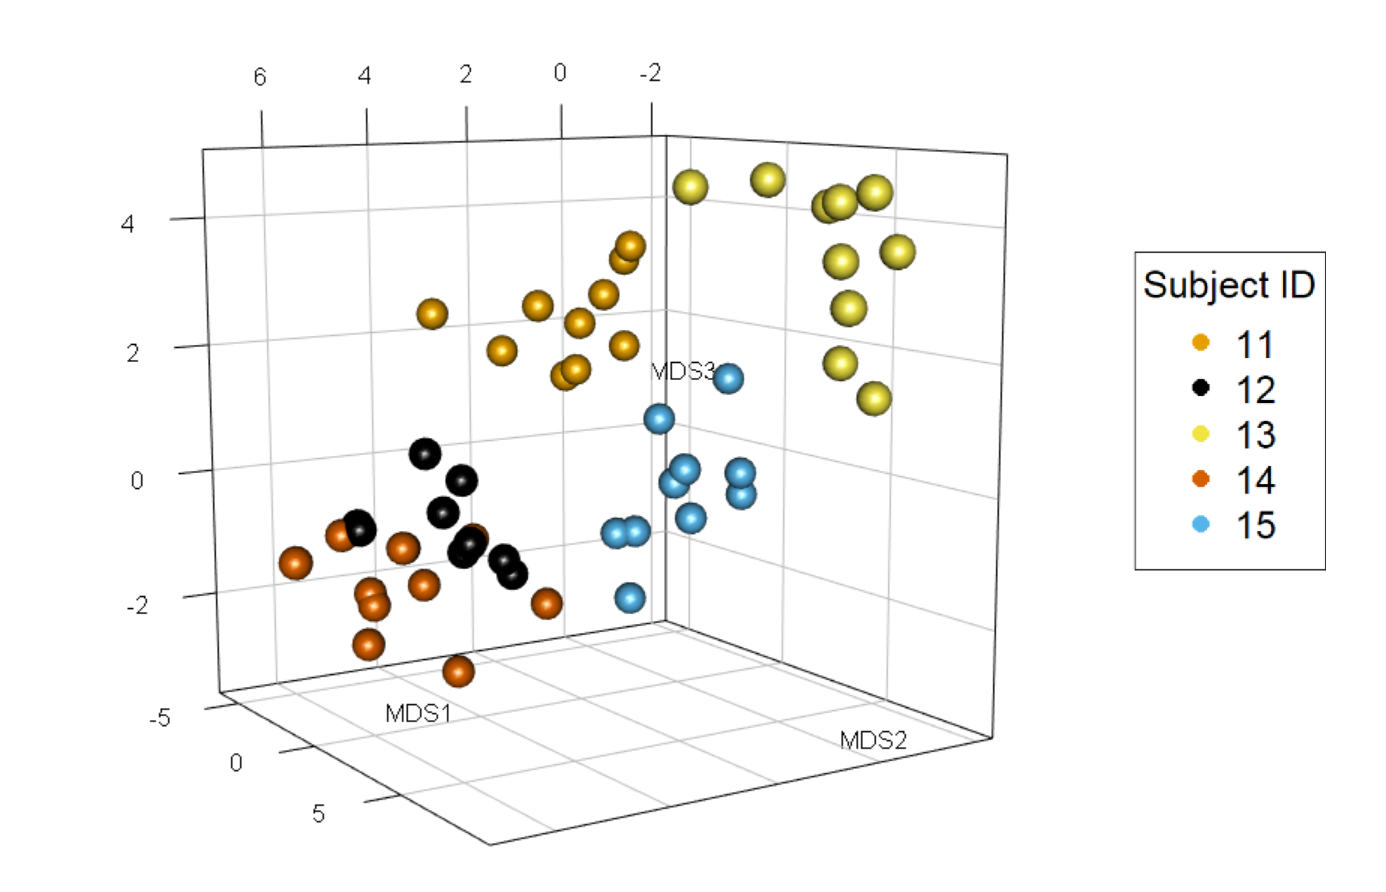
\includegraphics[width=\textwidth]{Images/HNU1-mds123-cbpalette}
					}\\					
				\end{minipage}
				
				\vspace{1cm}
			
			\begin{minipage}{0.58\textwidth}
				\centering
				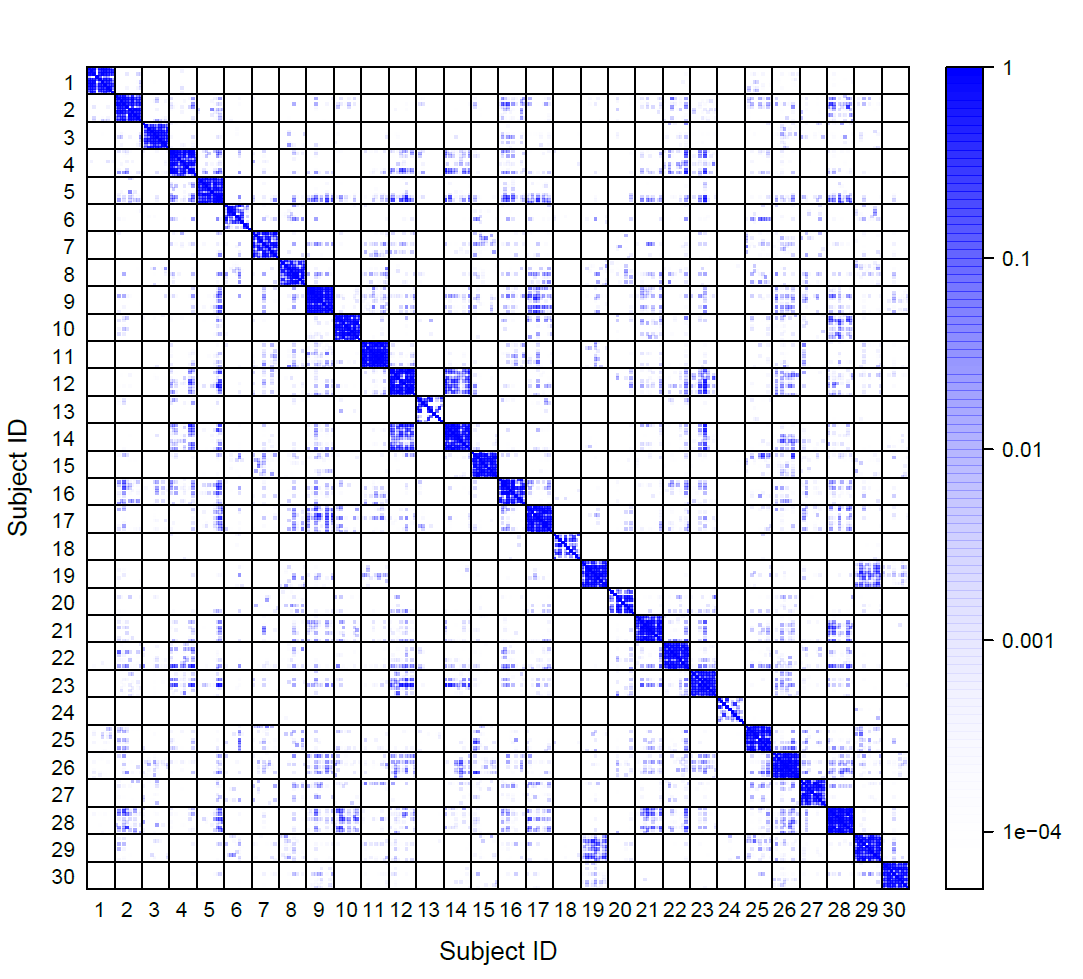
\includegraphics[width=1\textwidth]{Images/HNU1-pvals}
				{\footnotesize Matrix of p-values for the equal distribution test of every pair of graphs}
			\end{minipage}
			\begin{minipage}{0.4\textwidth}
				\textbf{Graph hypothesis testing}
				\begin{itemize}
					\item For each pair of graphs $i$ and $j$, we test the hypothesis that their distribution is the same, i.e., $H_0: \bR^{(i)} = \bR^{(j)}$ 
					\item Test statistic $\|\hat{\bR}^{(i)}-\hat{\bR}^{(j)}\|_F$
					\item Semiparametric bootstrap: estimate the parameters with MASE to sample new graphs
					\item The p-values of the test (left figure) are generally high for pairs of graphs from the same subject (diagonal entries) and low for different subjects
				\end{itemize}
			\end{minipage}

					
				}
		\end{Section}
		\begin{minipage}{0.43\textwidth}
			\begin{tcolorbox}[colback=blue!5,colframe=boxcol,title=Acknowledgements,width=\textwidth]
				{\footnotesize  This research has been supported by the Lifelong Learning Machines (L2M) program of the Defence Advanced Research Projects Agency (DARPA) via contract number HR0011-18-2-0025. This work is also supported in part by the D3M program of DARPA. We would like to thank Keith Levin and Elizaveta Levina for helpful discussions.\par
				}
				
			\end{tcolorbox}	
		\end{minipage}\hfill
		\begin{minipage}{0.53\textwidth}
			\begin{tcolorbox}[colback=blue!5,colframe=boxcol,title=References,width=1.1\textwidth]
				\bibliographystyle{ieee} % Plain referencing style
				{\footnotesize  \bibliography{Biblio}
				Open R source code for MASE is available at \url{https://github.
				com/jesusdaniel/mase}, and in the Python GraSPy package at \url{https://neurodata.io/graspy}.\par}
	
			\end{tcolorbox}	

		\end{minipage}
		
		
		
		
	\end{minipage}
	\hfill
\end{minipage}

\end{document}
